
%%
%% This is file `sample-sigconf.tex',
%% generated with the docstrip utility.
%%
%% The original source files were:
%%
%% samples.dtx  (with options: `sigconf')
%% 
%% IMPORTANT NOTICE:
%% 
%% For the copyright see the source file.
%% 
%% Any modified versions of this file must be renamed
%% with new filenames distinct from sample-sigconf.tex.
%% 
%% For distribution of the original source see the terms
%% for copying and modification in the file samples.dtx.
%% 
%% This generated file may be distributed as long as the
%% original source files, as listed above, are part of the
%% same distribution. (The sources need not necessarily be
%% in the same archive or directory.)
%%
%% The first command in your LaTeX source must be the \documentclass command.
\documentclass[sigconf]{acmart}

%%
%% \BibTeX command to typeset BibTeX logo in the docs
\AtBeginDocument{%
  \providecommand\BibTeX{{%
    \normalfont B\kern-0.5em{\scshape i\kern-0.25em b}\kern-0.8em\TeX}}}

%% Rights management information.  This information is sent to you
%% when you complete the rights form.  These commands have SAMPLE
%% values in them; it is your responsibility as an author to replace
%% the commands and values with those provided to you when you
%% complete the rights form.
%%\setcopyright{acmcopyright}
%%\copyrightyear{2018}
%%\acmYear{2018}
%%\acmDOI{10.1145/1122445.1122456}

%% These commands are for a PROCEEDINGS abstract or paper.
%%\acmConference[Woodstock '18]{Woodstock '18: ACM Symposium on Neural
%%  Gaze Detection}{June 03--05, 2018}{Woodstock, NY}
%%\acmBooktitle{Woodstock '18: ACM Symposium on Neural Gaze Detection,
%%  June 03--05, 2018, Woodstock, NY}
%%\acmPrice{15.00}
%%\acmISBN{978-1-4503-XXXX-X/18/06}


%%
%% Submission ID.
%% Use this when submitting an article to a sponsored event. You'll
%% receive a unique submission ID from the organizers
%% of the event, and this ID should be used as the parameter to this command.
%%\acmSubmissionID{123-A56-BU3}

%%
%% The majority of ACM publications use numbered citations and
%% references.  The command \citestyle{authoryear} switches to the
%% "author year" style.
%%
%% If you are preparing content for an event
%% sponsored by ACM SIGGRAPH, you must use the "author year" style of
%% citations and references.
%% Uncommenting
%% the next command will enable that style.
%%\citestyle{acmauthoryear}

%%
%% end of the preamble, start of the body of the document source.
\begin{document}

%%
%% The "title" command has an optional parameter,
%% allowing the author to define a "short title" to be used in page headers.
\title{Vulnerabilities in WebAssembly: A Survey}

%%
%% The "author" command and its associated commands are used to define
%% the authors and their affiliations.
%% Of note is the shared affiliation of the first two authors, and the
%% "authornote" and "authornotemark" commands
%% used to denote shared contribution to the research.
\author{Holger Klein}
%%\authornote{Both authors contributed equally to this research.}
%%\email{uaidx@student.kit.edu}
%%\orcid{1234-5678-9012}
%%\author{G.K.M. Tobin}
%%\authornotemark[1]
%%\email{webmaster@marysville-ohio.com}
\affiliation{%
  \institution{Karlsruhe Institute of Technology (KIT)}
%%  \streetaddress{P.O. Box 1212}
  \city{Karlsruhe}
%%  \state{Deutschland}
  \country{Germany}
%%  \postcode{43017-6221}
}


%%
%% By default, the full list of authors will be used in the page
%% headers. Often, this list is too long, and will overlap
%% other information printed in the page headers. This command allows
%% the author to define a more concise list
%% of authors' names for this purpose.
\renewcommand{\shortauthors}{Holger Klein}

%%
%% The abstract is a short summary of the work to be presented in the
%% article.
\begin{abstract}
  A clear and well-documented \LaTeX\ document is presented as an
  article formatted for publication by ACM in a conference proceedings
  or journal publication. Based on the ``acmart'' document class, this
  article presents and explains many of the common variations, as well
  as many of the formatting elements an author may use in the
  preparation of the documentation of their work.
\end{abstract}

%%
%% The code below is generated by the tool at http://dl.acm.org/ccs.cfm.
%% Please copy and paste the code instead of the example below.
%%

%%
%% Keywords. The author(s) should pick words that accurately describe
%% the work being presented. Separate the keywords with commas.
\keywords{binary exploits, Webassembly, IT Security}

%% A "teaser" image appears between the author and affiliation
%% information and the body of the document, and typically spans the
%% page.
\begin{teaserfigure}
  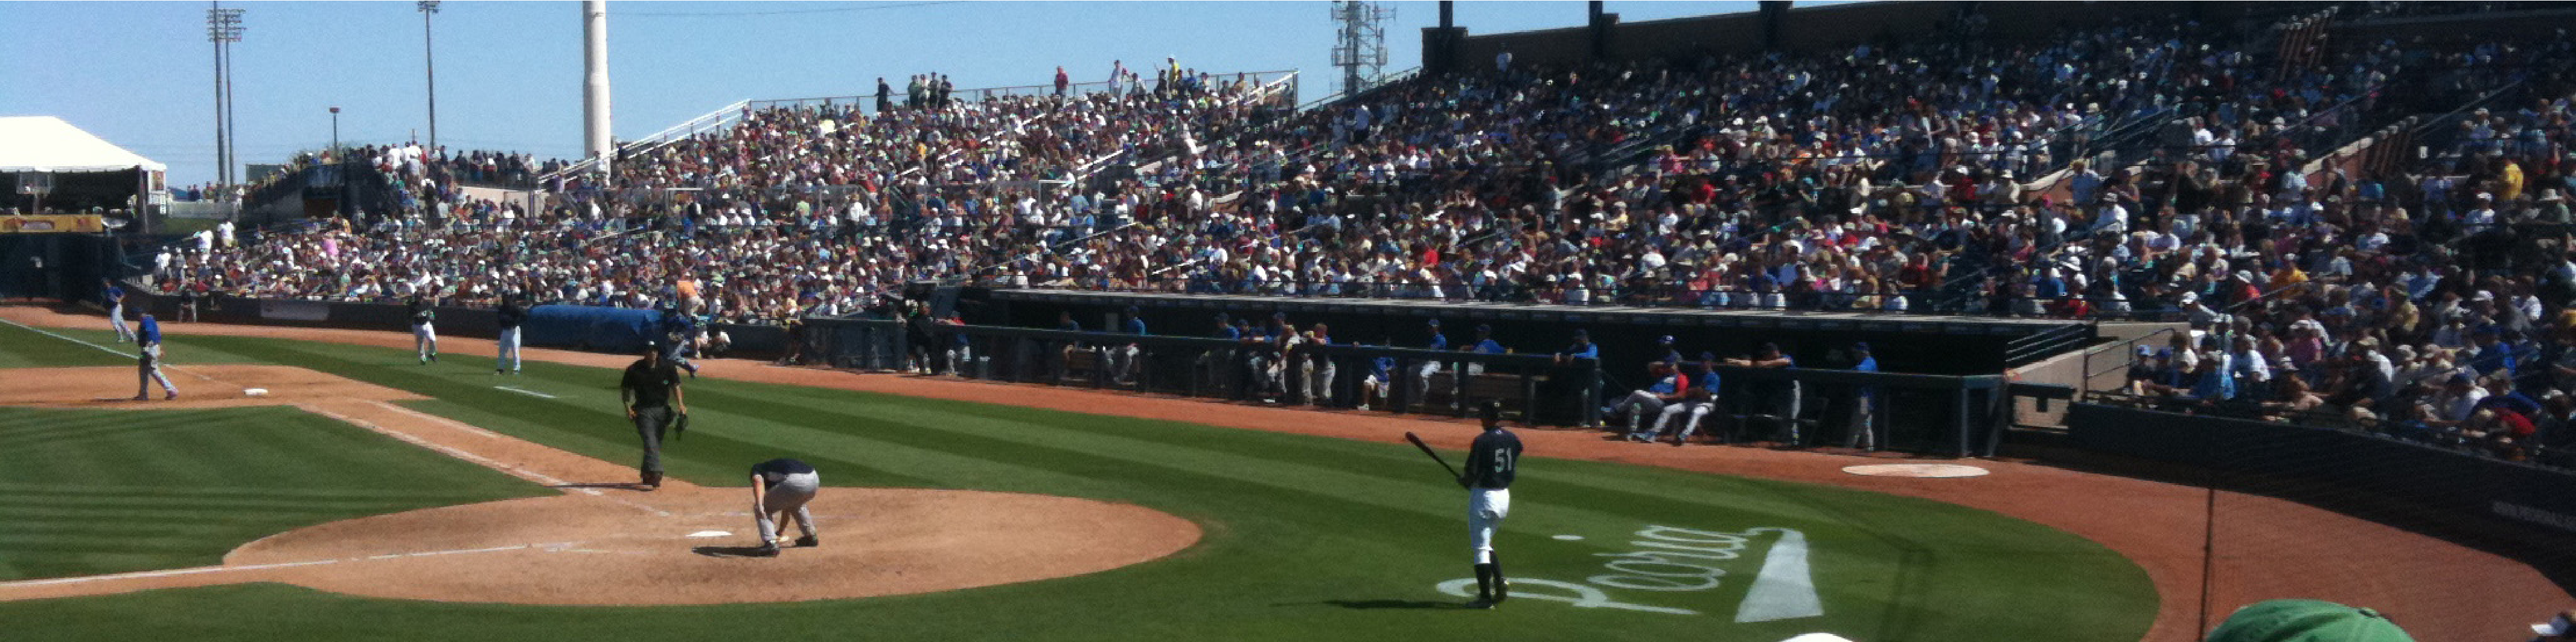
\includegraphics[width=\textwidth]{sampleteaser}
  \caption{Seattle Mariners at Spring Training, 2010.}
  \Description{Enjoying the baseball game from the third-base
  seats. Ichiro Suzuki preparing to bat.}
  \label{fig:teaser}
\end{teaserfigure}

%%
%% This command processes the author and affiliation and title
%% information and builds the first part of the formatted document.
\maketitle

\section{Introduction}
Introduce the papers structure: 
State of the art
What is wasm
	relevant features for vulnerabilities
What are binary exploitation techniques usually used 

Which can and cannot be used in wasm (picture/table?)
Talk about wasabi 
Talk about own experiments?

\cite{lehmann_everything_2020}

\section{WebAssembly}
The following will give an Introduction to and and overview of Webassembly, paying special attention to the parts relevant to a discussion of binary vulnerabilities. For more information, see the official specification at \cite{webAssembly_spec_2021}. 

\subsubsection{High Level Overview}
The name 'WebAssembly' (often abbreviated as WASM) is a slight misnomer, since it has a different form and function from typical assembly language formats. The official spec refers to it as "low-level, assembly-like". It is a binary byte code format which is interpreted by a Virtual Machine (similar to for example Java). The Virtual Machine is most often implemented in a browser. Design goals were to make WebAssembly safe, hardware- and language independent and fast. In fact, WebAssembly is supposed to run at near-native speeds. There exists a human-readable format of WebAssembly binaries called 'wat'. Whenever we show WebAssembly Code, it will be in this format.

\subsubsection{Modules}


\bibliographystyle{ACM-Reference-Format}
\bibliography{Wasm-Vuln}

%%
%% If your work has an appendix, this is the place to put it.
\appendix


\end{document}
\endinput
%%
%% End of file `sample-sigconf.tex'.'